\documentclass[a4paper,10pt]{article}
\usepackage[utf8]{inputenc}
\usepackage[english]{babel}
\usepackage{amsmath, amssymb, mathtools}
\usepackage{tikz}
\usetikzlibrary{patterns}
\usepackage{geometry}
\geometry{margin=1.7cm}
\usepackage{hyperref}
\usepackage{enumitem}
\usepackage{nicematrix}
\usepackage{eurosym} % para el euro
\setlength{\parindent}{0pt}
\title{Integer Linear Programming\\Algorithmic Methods for Mathematical Models}
\author{Elena de Paz Obiols}
\date{\today}
\usepackage{float}

\begin{document}


\maketitle

\section*{Problem 1: Food Production Optimization}

\subsection*{Problem Statement}

A food is manufactured by refining raw oils and blending them together. The raw oils come in two categories:

\textbf{Vegetable oil:} VEG 1, VEG 2

\textbf{Non-vegetable oil:} NON 1, NON 2, NON 3

Vegetable oils and non-vegetable oils require different production lines for refining. It is not possible to refine more than 200 tons of vegetable oil and more than 250 tons of non-vegetable oils. There is no loss of weight in the refining process and the cost of refining may be ignored.

There is a technological restriction of hardness in the final product. In the units in which hardness is measured, this must lie between 3 and 6. We assume the hardness of final product is the weighted average of hardness of the raw oils.

\textbf{Data:}
\begin{center}
\begin{tabular}{|c|c|c|c|c|c|}
\hline
& VEG 1 & VEG 2 & NON 1 & NON 2 & NON 3 \\
\hline
Hardness & 8.8 & 6.1 & 2.0 & 4.2 & 5.0 \\
\hline
Cost (\euro/ton) & 110 & 120 & 130 & 110 & 115 \\
\hline
\end{tabular}
\end{center}

The final product sells at 150{\euro} per ton.

\textbf{Additional conditions:}
\begin{itemize}
    \item The food should be made up of at least three oils.
    \item If an oil is used then at least 20 tons must be used.
    \item If either of VEG 1 or VEG 2 is used then NON 3 must also be used.
\end{itemize}

\textbf{Objective:} What manufacturing policy should the company pursue in order to maximize profit? Formulate the problem as an MIP.

\subsection*{Part (a): Basic LP Formulation}

\textbf{Decision variables:}
\begin{align}
TVEG_1, TVEG_2 &= \text{tons of vegetable oils VEG1, VEG2 used}\\
TNON_1, TNON_2, TNON_3 &= \text{tons of non-vegetable oils NON1, NON2, NON3 used}\\
PROD &= TVEG_1 + TVEG_2 + TNON_1 + TNON_2 + TNON_3 \text{ (total production)}
\end{align}

\textbf{Objective function:}
\begin{align}
\text{Maximize } Z = &150 \cdot PROD - 110 \cdot TVEG_1 - 120 \cdot TVEG_2 \\
&- 130 \cdot TNON_1 - 110 \cdot TNON_2 - 115 \cdot TNON_3
\end{align}

\textbf{Basic constraints:}
\begin{align}
&\text{Vegetable oil refining capacity: } TVEG_1 + TVEG_2 \leq 200\\
&\text{Non-vegetable oil refining capacity: } TNON_1 + TNON_2 + TNON_3 \leq 250\\
&\text{Minimum hardness: }\\
&\qquad \frac{8.8 \cdot TVEG_1 + 6.1 \cdot TVEG_2 + 2.0 \cdot TNON_1 + 4.2 \cdot TNON_2 + 5.0 \cdot TNON_3}{PROD} \geq 3\\
&\text{Maximum hardness: }\\
&\qquad \frac{8.8 \cdot TVEG_1 + 6.1 \cdot TVEG_2 + 2.0 \cdot TNON_1 + 4.2 \cdot TNON_2 + 5.0 \cdot TNON_3}{PROD} \leq 6\\
&\text{Total production definition: }\\
&\qquad PROD = TVEG_1 + TVEG_2 + TNON_1 + TNON_2 + TNON_3\\
&TVEG_1, TVEG_2, TNON_1, TNON_2, TNON_3 \geq 0
\end{align}

\subsection*{Part (b): MIP Formulation with Additional Conditions}

\textbf{Additional binary variables:}
\begin{align}
UVEG_1, UVEG_2 &= \begin{cases} 
1 & \text{if vegetable oil VEG1, VEG2 is used} \\
0 & \text{otherwise}
\end{cases}\\
UNON_1, UNON_2, UNON_3 &= \begin{cases} 
1 & \text{if non-vegetable oil NON1, NON2, NON3 is used} \\
0 & \text{otherwise}
\end{cases}
\end{align}

\textbf{Additional constraints for extra conditions:}
\begin{align}
&\text{At least 3 oils: } UVEG_1 + UVEG_2 + UNON_1 + UNON_2 + UNON_3 \geq 3\\
&\text{Minimum usage per oil: }\\
&\qquad TVEG_1 \geq 20 \cdot UVEG_1, \quad TVEG_2 \geq 20 \cdot UVEG_2\\
&\qquad TNON_1 \geq 20 \cdot UNON_1, \quad TNON_2 \geq 20 \cdot UNON_2, \quad TNON_3 \geq 20 \cdot UNON_3\\
&\text{Maximum usage per oil: }\\
&\qquad TVEG_1 \leq M \cdot UVEG_1, \quad TVEG_2 \leq M \cdot UVEG_2\\
&\qquad TNON_1 \leq M \cdot UNON_1, \quad TNON_2 \leq M \cdot UNON_2, \quad TNON_3 \leq M \cdot UNON_3\\
&\text{VEG→NON3 implication: } UVEG_1 + UVEG_2 \leq 2 \cdot UNON_3\\
&UVEG_1, UVEG_2, UNON_1, UNON_2, UNON_3 \in \{0,1\}
\end{align}



\subsection*{Binary Variable Transformations}

\textbf{How to find the transformations for binary variables?}

Let $b$ be a binary variable and $f(x)$ a linear expression.

\textbf{Case 1:} We want to express with linear inequalities that ``if $b=0$ then $f(x) \leq 0$'':

Let $U$ be an upper bound for the value of $f(x)$ over all feasible solutions. 
Then, for any feasible solution, the following constraint holds:
\[f(x) \leq U \cdot b\]
If $b=0$, then $f(x) \leq 0$. If $b=1$, then $f(x) \leq U$, which is always true.

\textbf{Case 2:} We want to express with linear inequalities that ``if $b=1$ then $f(x) \geq 0$'':

Let $L$ be a lower bound for the value of $f(x)$ over all feasible solutions.
Then, for any feasible solution, the following constraint holds:
\[f(x) \geq L \cdot (1-b)\]
If $b=1$, then $f(x) \geq 0$. If $b=0$, then $f(x) \geq L$, which is always true.
\\

In case we have ``if $b=0$ then $f(x) \geq k$'':
We can transform our function by defining a new function $f'(x) = f(x) - k$. Then, we can apply the same logic as in Case 2:
Let $L'$ be a lower bound for the value of $f'(x)$ over all feasible solutions.
Then, for any feasible solution, the following constraint holds:
\[f'(x) \geq L' \cdot (1-b)\]
Which can be rewritten as:
\[f(x) - k \geq L' \cdot (1-b)\]
or equivalently:
\[f(x) \geq k + L' \cdot (1-b)\]

\newpage

\section*{Problem 2: Sudoku}

Given the following Sudoku puzzle,

\begin{center}
\begin{NiceTabular}{|>{\centering\arraybackslash}m{0.35em}|>{\centering\arraybackslash}m{0.35em}|>{\centering\arraybackslash}m{0.35em}|!{\vrule width 1.2pt}>{\centering\arraybackslash}m{0.35em}|>{\centering\arraybackslash}m{0.35em}|>{\centering\arraybackslash}m{0.35em}|!{\vrule width 1.2pt}>{\centering\arraybackslash}m{0.35em}|>{\centering\arraybackslash}m{0.35em}|>{\centering\arraybackslash}m{0.35em}|}
\hline
5 & 3 &   &   & 7 &   &   &   &   \\
\hline
6 &   &   & 1 & 9 & 5 &   &   &   \\
\hline
  & 9 & 8 &   &   &   &   & 6 &   \\
\hline
8 &   &   &   & 6 &   &   &   & 3 \\
\hline
4 &   &   & 8 &   & 3 &   &   & 1 \\
\hline
7 &   &   &   & 2 &   &   &   & 6 \\
\hline
  & 6 &   &   &   &   & 2 & 8 &   \\
\hline
  &   &   & 4 & 1 & 9 &   &   & 5 \\
\hline
  &   &   &   & 8 &   &   & 7 & 9 \\
\hline
\end{NiceTabular}
\end{center}

formulate the problem of completing it as a MIP.
\subsection*{MIP Formulation}

\textbf{Decision variables:}
\begin{itemize}
  \item \(x_{ijk}\): binary variable that is 1 if the cell in row \(i\) and column \(j\) contains the number \(k\), and 0 otherwise.\\
  Where \(i, j, k \in \{1, 2, \ldots, 9\}\).
\end{itemize}

\textbf{Objective function:}
There is no objective function. To cost the problem as a MIP, we can take arbitrarily any function, for example: we can minimize 0.\\

\textbf{Constraints:}
\begin{enumerate}
  \item At each row, each value appears exactly once:
  \[
  \sum_{i=1}^{9} x_{ijk} = 1 \quad \forall j, k \in \{1, \ldots, 9\}
  \]
  \item At each column, each value appears exactly once:
  \[
  \sum_{j=1}^{9} x_{ijk} = 1 \quad \forall i, k \in \{1, \ldots, 9\}
  \]
  \item In each 3x3 subsquare, each value appears exactly once:\\

  Let's us identify each of the subsquares with the set of coordinates if its cells:
  \begin{itemize}
    \item $\mathbf{S_{11}} = \{(1,1), (1,2), (1,3), (2,1), (2,2), (2,3), (3,1), (3,2), (3,3)\}$ 
  \end{itemize}

  \[
    \begin{bmatrix}
      S_{11} & S_{12} & S_{13} \\
      S_{21} & S_{22} & S_{23} \\
      S_{31} & S_{32} & S_{33} \\
    \end{bmatrix}
  \]

  For each subsquare S, for all values k:
  \[\sum_{(i,j) \in S} x_{ijk} = 1 \quad \forall k \in \{1, \ldots, 9\}\]

  \item Fixed cells are respected. \\
  For each fixed cell (i,j) with value k:
  \[x_{ijk} = 1\]

  \item At each cell (i,j), there is exactly one value:
  \[\sum_{k=1}^{9} x_{ijk} = 1 \quad \forall i, j \in \{1, \ldots, 9\}\]

\end{enumerate}

\newpage

\section*{Problem 3: Twenty-Seven Cells Arrangement}

\subsection*{Problem Statement}
Twenty-seven cells are arranged in a three-dimensional 3 × 3 × 3 cube as shown below. 

\begin{center}

\includegraphics[width=0.4\textwidth]{rubik_cube.png}
\end{center}

Three cells are regarded as lying in the same line if they are on the same horizontal or vertical line or the same diagonal. Diagonals exist on each horizontal and vertical section and connecting opposite vertices of the cube. (There are 49 lines altogether.)

Given 13 white balls and 14 black balls, arrange them, one to a cell, so as to minimise the number of lines with balls all of one colour.

\subsection*{MIP Formulation}

Let's identify each of the three cells in the cube with a triplet \((i,j,k)\) where \(i,j,k \in \{0,1,2\}\).\\
Moreover, let's identify a line with the set of coordinates of its cells.\\

\begin{center}
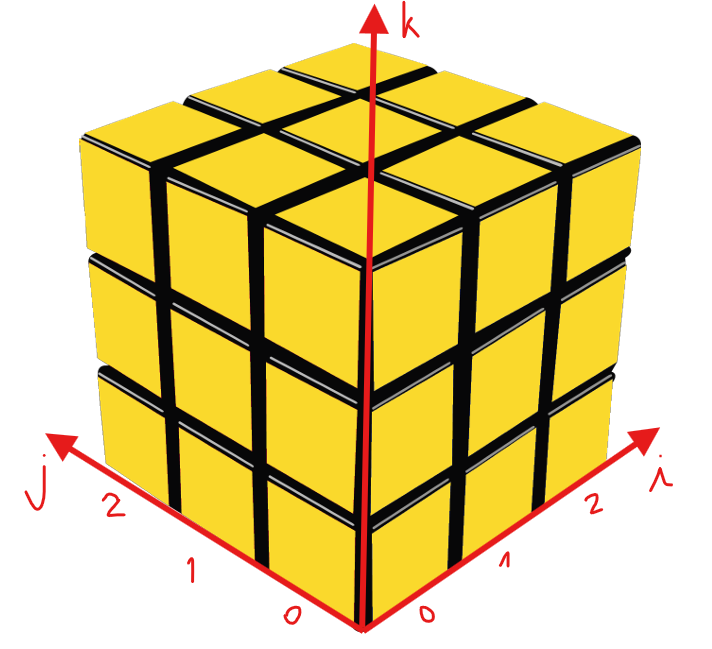
\includegraphics[width=0.3\textwidth]{rubik_con_ejes.png}
\end{center}

\textbf{Decision variables:}
\begin{itemize}
  \item \(x_{ijk}\) = the ball at cell \((i,j,k)\) is white (1) or black (0).\\
  Where \(i, j, k \in \{0, 1, 2\}\). (of type binary)
  \item \(y_l\) = the ball in line \(l\) are all of the same color (1) or not (0).\\
  Where \(l \in \{1, 2, \ldots, 49\}\) (the 49 lines in total). (of type binary) 
\end{itemize}

\textbf{Objective function:}
Minimize the number of lines with balls all of one colour:
\[\text{minimize } \sum_{l=1}^{49} y_l\]

\textbf{Constraints:}

\begin{enumerate}
  \item There are 13 white balls and 14 black balls:
  \begin{align}
  \boxed{\sum_{(i,j,k) \in \text{cells}} x_{ijk} = 13} \quad \text{and} \quad 
  \boxed{\sum_{(i,j,k) \in \text{cells}} (1 - x_{ijk}) = 14}
  \end{align}
  \item If all balls in a line \(l\) have the same colour, then \(y_l = 1\).\\
  Let \(l\) be the line consisting of the cells \((i_0,j_0,k_0), (i_1,j_1,k_1), (i_2,j_2,k_2)\).
  Let's consider two cases:
  \begin{enumerate}
    \item If all balls in line \(l\) are \textbf{white} , then \(y_l=1\) :
      \[x_{i_0 j_0 k_0} \land x_{i_1 j_1 k_1} \land x_{i_2 j_2 k_2} \Rightarrow y_l\]
      \[\lnot (x_{i_0 j_0 k_0} \land x_{i_1 j_1 k_1} \land x_{i_2 j_2 k_2}) \lor y_l \quad \text{(by implication law)}\]

      \textcolor{gray}{If \(a_1, a_2, \dots, a_n, b_1, b_2, \dots, b_m\) are binary variables, then:
        \[
          \lnot (a_1 \land a_2 \land \dots \land a_n) \lor (b_1 \land b_2 \land \dots \land b_m) \Leftrightarrow \sum_{i=1}^{n} (1 - a_i) + \sum_{j=1}^{m} b_j \geq 1
        \]}
      Therefore, we can express our constraint as:
      \[\boxed{(1 - x_{i_0 j_0 k_0}) + (1 - x_{i_1 j_1 k_1}) + (1 - x_{i_2 j_2 k_2}) + y_l \geq 1}\]
    
      \item If all balls in line \(l\) are \textbf{black} , then \(y_l=1\) :
      \[(1 - x_{i_0 j_0 k_0}) \land (1 - x_{i_1 j_1 k_1}) \land (1 - x_{i_2 j_2 k_2}) \Rightarrow y_l\]
      \[
        \lnot ((1 - x_{i_0 j_0 k_0}) \land (1 - x_{i_1 j_1 k_1}) \land (1 - x_{i_2 j_2 k_2})) \lor y_l
      \]
      Applying the same reasoning as in the previous case, we can express our constraint as:
      \[\boxed{x_{i_0 j_0 k_0} + x_{i_1 j_1 k_1} + x_{i_2 j_2 k_2} + y_l \geq 1}\]
  \end{enumerate}
\end{enumerate}

\newpage

\section*{Problem 4: Infectious Disease Outbreak Investigation}

\subsection*{Problem Statement}
An outbreak of an infectious disease has been observed in a set $N$ of locations. There exists a set $M$ of teams capable of investigating these outbreaks. Team $i \in M$ can conclude its investigation of the outbreak in location $j \in N$ in $t_{ij}$ hours. Each team can either investigate zero, one, or two outbreaks. If a team investigates two outbreaks, they must travel from one location to the next. The travel time from location $j_1 \in N$ to location $j_2 \in N$ is $d_{j_1 j_2}$. Travel times can be assumed to be symmetric. Once all outbreaks have been investigated, a disease control center can take action to combat the outbreak. The goal is to minimize the amount of time necessary to complete the investigation of all locations.

\subsection*{MIP Formulation}
\textbf{Decision variables:}
\begin{itemize}
  \item \(x_{ij}\) = 1 if team \(i\) investigates location \(j\), 0 otherwise.\\
  Where \(1 \leq i \leq M\) and \(1 \leq j \leq N\). (of type binary)
  \item \(y_{ij_1j_2}\) = 1 if team \(i\) investigates locations \(j_1\) and \(j_2\) in that order, 0 otherwise.\\
  Where \(1 \leq i \leq M\) and \(1 \leq j_1, j_2 \leq N\). (of type binary)
  \item z = the maximum time needed for any team to complete its investigations. (of type real non negative)
\end{itemize}

\textbf{Constraints:}
\begin{enumerate}
  \item Each team can investigate at most two locations:
  \[\boxed{
  \sum_{j=1}^N x_{ij} \leq 2 \quad \forall 1 \leq i \leq M}
  \]
  \item Each location must be investigated by exactly one team:
  \[
  \boxed{\sum_{i=1}^M x_{ij} = 1 \quad \forall 1 \leq j \leq N}
  \]
  \item Variables are linked: \(y_{ij_1j_2} \iff (x_{ij_1} \land x_{ij_2})\):
  \begin{enumerate}
    \item  \(y_{ij_{1j_2} } \implies (x_{ij_1} \land x_{ij_2})\):
    \[ \lnot y_{ij_1 j_2} \lor (x_{ij_1} \land x_{ij_2}) \]
    \[ (\lnot y_{ij_1 j_2} \lor x_{ij_1}) \land (\lnot y_{ij_1 j_2} \lor x_{ij_2}) \]
    \[(1-y_{ij_1 j_2}) + x_{ij_1} \geq 1 \text{ and } (1-y_{ij_1 j_2}) + x_{ij_2} \geq 1\]
    Therefore, we can express our constraints as:
    \[
      \boxed{y_{ij_1 j_2} \leq x_{ij_1}} \quad \text{and} \quad \boxed{y_{ij_1 j_2} \leq x_{ij_2}} \quad \forall 1 \leq i \leq M, 1 \leq j_1, j_2 \leq N
    \]
    \item \(y_{ij_{1j_2} } \impliedby (x_{ij_1} \land x_{ij_2})\):
    \[ (x_{ij_1} \land x_{ij_2}) \implies y_{ij_1 j_2} \]
    \[ \lnot (x_{ij_1} \land x_{ij_2}) \lor y_{ij_1 j_2} \]
    \[ \lnot x_{ij_1} \lor \lnot x_{ij_2} \lor y_{ij_1 j_2} \]
    \[ (1 - x_{ij_1}) + (1 - x_{ij_2}) + y_{ij_1 j_2} \geq 1 \]
    Therefore, we can express our constraint as:
    \[
      \boxed{x_{ij_1} + x_{ij_2} - y_{ij_1 j_2} \leq 1} \quad \forall 1 \leq i \leq M, 1 \leq j_1, j_2 \leq N 
    \]
  \end{enumerate}

  \item z has its intended meaning:
  For every team \(i\), the time needed for team \(i\) to complete its investigations must be less than or equal to \(z\):
  \[\boxed{\sum_{j=1}^N t_{ij} x_{ij} + \sum_{\substack{j_1,j_2=1 \frac{}{} j_1<j_2}}^{N} d_{j_1 j_2} \cdot y_{i j_1 j_2} \leq z \quad \forall 1 \leq i \leq M}\]

\end{enumerate}

\textbf{Objective function:}
Minimize the time needed to complete the investigation of all locations.\\
\[
  \min \max _{1 \leq i \leq M} \left\{ \text{time needed for team } i \right\}
\]
The time needed for team \(i\) to complete its investigations is
\[\sum_{j=1}^N t_{ij} x_{ij} + \sum_{j_1=1}^N \sum_{j_2=1}^N d_{j_1 j_2} (x_{i j_1} \wedge x_{i j_2}) \implies \sum_{\substack{j_1,j_2=1 \\ j_1<j_2}}^{N} d_{j_1 j_2} \cdot y_{i j_1 j_2}\]

\newpage
\section*{Problem 5: Graph Coloring}

\subsection*{Problem Statement}
Consider the problem of graph coloring: given a graph $G = (V,E)$, we want to find the minimum number of colors to paint the vertices so that adjacent vertices have different colors. Model this problem as a MIP.

\subsection*{MIP Formulation}

Let's label vertices $1, 2, \dots, n = |V|$.\\

\textbf{Decision variables:}
\begin{itemize}
  \item \(c_v\) = color assigned to vertex \(v\) (for all \(v \in V\)) (of type integer non negative)
  \item \(z\) = intuitively, \(\max_{v \in V} c_v\) (of type integer non negative)
  \item \(z_{uv}\) = 1 if \(c_u < c_v\), 0 if \(c_u > c_v\) (for all \((u,v) \in E\)) (of type binary)
\end{itemize}

\textbf{Objective function:}
Minimize the number of colors used:
\[\min z\]

\textbf{Constraints:}
\begin{enumerate}
  \item \(z\) 'behaves' as \(\max_{v \in V} c_v\):
  \[\boxed{c_v \leq z \quad \forall v \in V}\] 
  \item Adjacent vertices have different colors:
  \[\boxed{c_u \neq c_v \quad \forall (u,v) \in E}\]
  The problem is that this equation is not linear. We can transform it using binary variables:
  
  This is the same as saying that either \(c_u < c_v\) or \(c_u > c_v\) \(\implies\) \(c_u +1 \leq c_v \lor c_u \geq c_{v}+1 \)  

  We define a new variable \(z_{uv}\) such that:
  \[z_{uv} = \begin{cases}
    1 & \text{if } c_u < c_v \\
    0 & \text{if } c_u > c_v
  \end{cases}\]

  We can express our constraint as:
  \[
  z_{uv} = 1 \implies c_u + 1 \leq c_v \implies c_v - c_u -1 \geq 0
  \]
  \[
  z_{uv} = 0 \implies c_u \geq c_v + 1 \implies c_u - c_v -1 \geq 0
  \]

  Applying the transformations for binary variables explained in Problem 1, we get:

  If \(b=0 \longrightarrow f(x) \leq 0 \text{ is equivalent to } \) \(f(x) \leq U \cdot b\), where \(U\) is an upper bound for \(f(x)\).

  If \(b=1 \longrightarrow f(x) \geq 0 \text{ is equivalent to } \) \(f(x) \geq L \cdot (1-b)\), where \(L\) is a lower bound for \(f(x)\).

  \begin{itemize}
    \item Let's express \(z_{uv}=1 \implies c_{v} - c_u - 1 \geq 0\)
  We know that \(c_v \geq 1 \implies c_u \leq n \implies -c_u \geq -n\)
  
  Therefore, a lower bound is \(L = -n\).

  So, the implication is equivalent to:
  \[c_v - c_u - 1 \geq -n \cdot (1 - z_{uv})\]

    \item Let's express \(z_{uv}=0 \implies c_u - c_v - 1 \geq 0\)
  We know that \(c_v \leq n \implies c_u \geq 1 \implies -c_u \leq -1\)

  Therefore, an upper bound is \(U=n\).

  So, the implication is equivalent to:
  \[c_u - c_v - 1 \leq n \cdot z_{uv}\]
  \end{itemize}

  Therefore, we can express our constraints as:
  \[
  \boxed{c_v - c_u - 1 \geq -n \cdot (1 - z_{uv})} \quad \text{and} \quad \boxed{c_u - c_v - 1 \leq n \cdot z_{uv}} \quad \forall (u,v) \in E
  \]  

\end{enumerate}

\subsection*{Alternative MIP Formulation}

Another possibility of defining the decision variables is:
\begin{itemize}
  \item \(x_{vc}\) = 1 if vertex \(v\) is assigned color \(c\), 0 otherwise (for all \(v \in V\) and \(1 \leq c \leq n\)) (of type binary)
  \item \(u_k\) = 1 if color \(k\) is used, 0 otherwise (for all \(1 \leq k \leq n\)) (of type binary)
  \item \(z\) = number of colors used (of type integer non negative) 
\end{itemize}

\textbf{Objective function:}
Minimize the number of colors used: 
\[
\min z
\]

\textbf{Constraints:}
\begin{enumerate}
  \item Variables are related:
  For each \(1 \leq v \leq n\) and \(1 \leq k \leq n\):
  \[x_{vk} \rightarrow u_k \quad \implies \quad \lnot x_{vk} \lor u_k \quad \implies \quad (1 - x_{vk}) + u_k \geq 1 \quad \implies \quad \boxed{u_k \geq x_{vk}}\]

  \item Neighbors are painted with different colors:
  For each edge \((u,v) \in E\) and \(1 \leq k \leq n\):
  \[
    \lnot (x_{uk} \land x_{vk}) \quad \implies \quad (1 - x_{uk}) + (1 - x_{vk}) \geq 1 \quad \implies \quad \boxed{x_{uk} + x_{vk} \leq 1}
  \]

  \item Each vertex is painted with exactly one color:
  For each \(1 \leq v \leq n\):
  \[\boxed{\sum_{k=1}^n x_{vk} = 1}\]

  \textbf{Observation}: This constraint was not in our first formulation because it was implicit in the definition of the variables \(c_v\).

\end{enumerate}

\newpage

\section*{Problem 6: Medical Drug Acquisition Planning}

\subsection*{Problem Statement}
A medical company is attempting to acquire a certain drug from a set M of suppliers. The company requires $d_t$ units of this drug in month $t$, for $t = 1, \ldots, T$, which are entirely consumed. Purchasing one unit of the drug from supplier $i \in M$ during time period $t \in \{1, \ldots, T\}$ costs $c_{it}$ (in \euro). However, in order to purchase drugs from supplier $i \in M$, at any time period, the company must purchase a minimum of $\ell_i$ units during that time period. Fortunately, if it turns out that there is more drug than required, the company can store at most $h$ units from one period to the next. If even then the company finds itself with too many units of the drug, it can simply throw away the extra supply. The goal is to minimize the cost required to purchase the drug for time periods $1, \ldots, T$.

\subsection*{MIP Formulation}

\textbf{Decision variables:}
\begin{itemize}
  \item \(x_{ijt}\) = number of units of drug purchased from supplier \(i\) at time period \(t\) (for all \(1 \leq i \leq M \text{ and }  1 \leq t \leq T\)) (of type integer non negative)
  \item \(y_t\) = number of units of drug stored at the end of time period \(t\) (for all \(1 \leq t \leq T-1\)) (of type integer non negative) (for convinience, we define \(y_0 = 0\)) 
  \item \(z_{it}\) = 1 if we purchase drugs from supplier \(i\) at time period \(t\), 0 otherwise (for all \(1 \leq i \leq M \text{ and }  1 \leq t \leq T\)) (of type binary) 
\end{itemize}

\textbf{Objective function:} 
Minimize costs: 
\[
  \min \sum_{\substack{1 \leq i \leq M \\ 1 \leq t \leq T}} c_{it} \cdot x_{it}
\]

\textbf{Constraints:} 
\begin{enumerate}
  \item At every period \(t\), the demand \(d_t\) must be satisfied:
    \begin{align*}
      &\text{For period } t=1: & \sum_{i=1}^M x_{i1} &\geq d_1 \\
      &\text{For period } t=2: & \sum_{i=1}^M x_{i2} + y_{1} &\geq d_2 + y_{2}\\
      &\vdotswithin{=} \\
      &\text{For period } t=T: & \sum_{i=1}^M x_{iT} + y_{T-1} &\geq d_T + y_{T}
    \end{align*}

  We can express our constraints as:
  \[\boxed{\sum_{i=1}^M x_{it} + y_{t-1} \geq d_t + y_t \quad \forall 1 \leq t \leq T}\]

  \textit{Explanation of the constraint}: the total amount of drug available at period \(t\) (the amount purchased at period \(t\) plus the amount stored from the previous period) must be greater than or equal to the total amount of drug needed at period \(t\) (the amount required at period \(t\) plus the amount stored for the next period).

  \item The storage capacity is limited:
  \[\boxed{y_t \leq h \quad \forall 1 \leq t \leq T}\]

  \item The purchase of drugs respect the minimum order quantity:
  For all \(1 \leq i \leq M\) and \(1 \leq t \leq T\):

  'If we buy drugs from supplier \(i\) at time period \(t\), then we must buy at least \(\ell_i\) units' can be expressed as:
  \[
    z_{it} = 0 \rightarrow x_{it} \leq 0 \quad \text{and} \quad z_{it} = 1 \rightarrow x_{it} \geq \ell_i
  \]

  Applying the transformations for binary variables, we get:
  \[
    \boxed{x_{it} \leq U_{iz} \cdot z_{it}} \quad \text{and} \quad \boxed{x_{it} \geq \ell_i \cdot z_{it}} \quad \forall 1 \leq i \leq M, 1 \leq t \leq T
  \]
  Where \(U_{iz}\) is an upper bound for the value of \(x_{it}\) over all feasible solutions. A possible value for \(U_{iz}\) is \(\sum_{t=1}^T d_t\).


\end{enumerate}


\newpage

\section*{Problem 7: Nurse Scheduling Problem}

\subsection*{Problem Statement}
A nurse is assigned a set $N$ of patients. For each patient $i \in N$, the nurse must spend $p_i$ minutes examining the patient. The nurse must then wait somewhere between $\ell_i$ and $u_i$ minutes before checking up on the patient, which requires $q_i$ minutes. The nurse, of course, cannot be in two places at the same time, although we will assume for simplicity that the travel time to walk from one patient's room to another is zero. The objective is to minimize the total amount of time required to tend to all patients.

\subsection*{MIP Formulation}

\textbf{Decision variables:}

\begin{itemize}
  \item \(f_i\) = time the first visit to patient \(i\) starts (for all \(i \in N\)) (of type real non negative)
  \item \(s_i\) = time the second visit to patient \(i\) starts (for all \(i \in N\)) (of type real non negative)
  
  \item \(ff_{ij}\) = 1st visit to patient \(i\) is before 1st visit to patient \(j\), (for all \(i, j \in N, i < j\)) (of type binary) 
  \item \(fs_{ij}\) = 1st visit to patient \(i\) is before 2nd visit to patient \(j\), (for all \(i, j \in N\)) (of type binary)
  \item \(sf_{ij}\) = 2nd visit to patient \(i\) is before 1st visit to patient \(j\), (for all \(i, j \in N\)) (of type binary)
  \item \(ss_{ij}\) = 2nd visit to patient \(i\) is before 2nd visit to patient \(j\), (for all \(i, j \in N, i < j\)) (of type binary)
\end{itemize}

\textbf{Constraints:} 
\begin{enumerate}
  \item The rest between visits is respected:
    \[\boxed{\ell_i \leq s_i - (f_i + p_i) \leq u_i \quad \forall i \in N}\]

    \begin{center}
      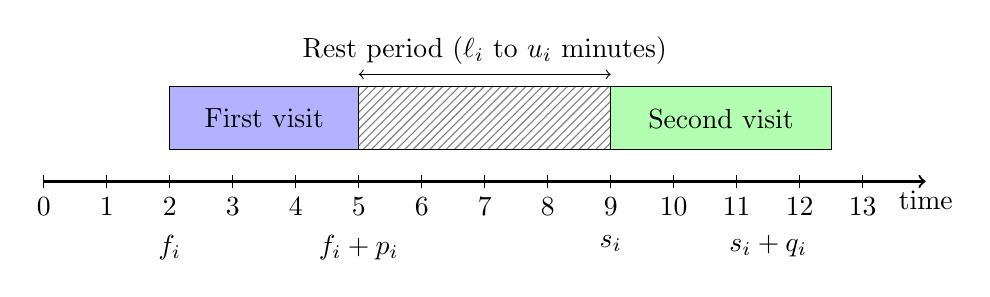
\begin{tikzpicture}[scale=0.8]
        % Timeline
        \draw[->, thick] (0,0) -- (14,0);
        \foreach \x in {0,1,...,13}
        \draw (\x,0.1) -- (\x,-0.1) node[below] {\x};
        \node[below] at (14,0) {time};
        
        % First visit
        \draw[fill=blue!30] (2,0.5) rectangle node {First visit} (5,1.5);
        
        % Rest period
        \draw[pattern=north east lines, pattern color=gray] (5,0.5) rectangle (9,1.5);
        \draw[<->] (5,1.7) -- node[above] {Rest period ($\ell_i$ to $u_i$ minutes)} (9,1.7);
        
        % Second visit
        \draw[fill=green!30] (9,0.5) rectangle node {Second visit} (12.5,1.5);
        
        % Labels
        \node[below] at (2,-0.7) {$f_i$};
        \node[below] at (5,-0.7) {$f_i + p_i$};
        \node[below] at (9,-0.7) {$s_i$};
        \node[below] at (11.5,-0.7) {$s_i + q_i$};
      \end{tikzpicture}
      \end{center}

    \textbf{Explanation:}
    \begin{itemize}
      \item $f_i$ = Time when first visit to patient $i$ starts
      \item $p_i$ = Duration of first visit (examination)
      \item $f_i + p_i$ = Time when first visit ends
      \item $s_i$ = Time when second visit (check-up) starts
      \item $s_i - (f_i + p_i)$ = Rest time between visits
      \item This rest time must be between $\ell_i$ and $u_i$ minutes
    \end{itemize}

    \item There are no overlapping visits:
    
    For each pair of patients \(i, j \in N\) with \(i < j\), we have four possible cases:
    \begin{enumerate}
      \item First visit to patient \(i\) ends before first visit to patient \(j\) starts:
      % \[f_i + p_i \leq f_j\]
      \item First visit to patient \(j\) ends before first visit to patient \(i\) starts:
      % \[f_j + p_j \leq f_i\]
      \item Second visit to patient \(i\) ends before second visit to patient \(j\) starts:
      % \[s_i + q_i \leq s_j\]
      \item Second visit to patient \(j\) ends before second visit to patient \(i\) starts:
      % \[s_j + q_j \leq s_i\]
    \end{enumerate}

    We will define four binary variables to represent these cases. See in the decision variables section.
    
    Therefore, we can express our constraints as:

    \[
      ff_{ij} + ff_{ji} = 1 \quad \forall i, j \in N, i < j
    \]
    \[
      ss_{ij} + ss_{ji} = 1 \quad \forall i, j \in N, i < j
    \]
    \[
      fs_{ij} + sf_{ji} = 1 \quad \forall i, j \in N, i \neq j
    \]

    \item The binary variables are linked to the time variables:
    \begin{enumerate}
      \item \(ff_{ij} = 1 \rightarrow f_i + p_i \leq f_j\):
      \[f_i + p_i \leq f_j + U \cdot (1 - ff_{ij})\]
      Where \(U\) is an upper bound for the value of \(f_j - (f_i + p_i)\) over all feasible solutions. A possible value for \(U\) is \(\sum_{i \in N} (p_i + u_i + q_i)\).

      \item \(ss_{ij} = 1 \rightarrow s_i + q_i \leq s_j\):
      \[s_i + q_i \leq s_j + U \cdot (1 - ss_{ij})\]
      Where \(U\) is an upper bound for the value of \(s_j - (s_i + q_i)\) over all feasible solutions. A possible value for \(U\) is \(\sum_{i \in N} (p_i + u_i + q_i)\).

      \item \(fs_{ij} = 1 \rightarrow f_i + p_i \leq s_j\):
      \[f_i + p_i \leq s_j + U \cdot (1 - fs_{ij})\]
      Where \(U\) is an upper bound for the value of \(s_j - (f_i + p_i)\) over all feasible solutions. A possible value for \(U\) is \(\sum_{i \in N} (p_i + u_i + q_i)\).

      \item \(sf_{ij} = 1 \rightarrow s_i + q_i \leq f_j\):
      \[s_i + q_i \leq f_j + U \cdot (1 - sf_{ij})\]
      Where \(U\) is an upper bound for the value of \(f_j - (s_i + q_i)\) over all feasible solutions. A possible value for \(U\) is \(\sum_{i \in N} (p_i + u_i + q_i)\).
    \end{enumerate}
  
\end{enumerate}

\textbf{Objective function:} 

Maximize the total profit:
\[\max \sum_{m \in M} \sum_{i \in P} \text{Profit}_i \cdot x_{i,m}\]

\newpage

\section*{Problem 8. Factories}

A company has two factories, one at Liverpool and one at Brighton. In addition, it has four depots with storage facilities at Newcastle, Birmingham, London and Exeter. The company sells its product to six customers C1, C2, ..., C6. Customers can be supplied from a or
the factory directly.

The distribution costs are known; they are given in the table below (in pounds per ton delivered). A dash in the table indicates the impossibility of certain suppliers for certain depots or customers.

\begin{center}
\begin{tabular}{|c|c|c|c|c|c|c|}
\hline
& Liverpool & Brighton & Newcastle & Birmingham & London & Exeter\\
\hline
Newcastle & 0.5 & - &&&& \\
Birmingham & 0.5 & 0.3 &&&& \\
London & 1.0 & 0.5 &&&& \\
Exeter & 0.2 & 0.2 &&&& \\
\hline
C1 & 1.0 & 2.0 & - & 1.0 & - & - \\
C2 & - & - & 1.5 & 0.5 & 1.5 & - \\
C3 & 1.5 & - & 0.5 & 0.5 & 2.0 & 0.2 \\
C4 & 2.0 & - & 1.5 & 1.0 & - & 1.5 \\
C5 & - & - & - & 0.5 & 0.5 & 0.5 \\
C6 & 1.0 & - & 1.0 & - & 1.5 & 1.5 \\
\hline
\end{tabular}
\end{center}

Each factory has a monthly capacity given as follows, which cannot be exceeded:
\begin{table}[H]
\centering
\begin{tabular}{|c|c|}
\hline
Factory & Monthly Capacity \\ 
\hline
Liverpool & 150,000 tons \\ 
Brighton & 200,000 tons \\ 
\hline
\end{tabular}
\caption{Monthly Capacity for Each Factory}
\end{table}

Each depot has a maximum monthly throughput given as follows, which cannot be exceeded:
\begin{table}[H]
\centering
\begin{tabular}{|c|c|}
\hline
Depot & Maximum Monthly Throughput \\
\hline
Newcastle & 70,000 tons \\
Birmingham & 50,000 tons \\
London & 100,000 tons \\
Exeter & 40,000 tons \\
\hline
\end{tabular}
\caption{Maximum Monthly Throughput for Each Depot}
\end{table}

Each customer has a monthly requirement given as follows, which must be met:
\begin{table}[H]
\centering
\begin{tabular}{|c|c|}
\hline
Customer & Monthly Requirement \\ 
\hline
C1 & 50,000 tons \\ 
C2 & 10,000 tons \\ 
C3 & 40,000 tons \\ 
C4 & 35,000 tons \\ 
C5 & 60,000 tons \\ 
C6 & 20,000 tons \\ 
\hline
\end{tabular}
\caption{Monthly Requirements for Each Customer}
\end{table}

(a) The company would like to determine what distribution pattern minimises overall cost.
Formulate the problem as an LP.

(b) There is a possibility of opening new depots at Bristol and Northampton, as well as of
enlarging the Birmingham depot.
It is not considered desirable to have more than four depots, and if necessary Newcastle or
Exeter (or both) can be closed down.
The monthly costs (in interest charges) of the possible new depots and expansion at Birmingham are given in the table below together with the potential monthly throughputs.
\begin{table}[H]
\centering
\begin{tabular}{|c|c|c|}
\hline
Depot & Monthly Cost (1000 pounds) & Monthly Throughput (1000 tons) \\ 
\hline
Bristol & 12 & 30 \\ 
Northampton & 4 & 25 \\ 
Birmingham (expansion) & 3 & 20 \\ 
\hline
\end{tabular}
\caption{Monthly Costs and Throughput for New Depots and Expansion}
\end{table}

The monthly savings of closing down the Newcastle and Exeter depots are given in the
following table:
\begin{table}[H]
\centering
\begin{tabular}{|c|c|}
\hline
Depot & Monthly Savings (1000 pounds) \\ 
\hline
Newcastle & 10 \\ 
Exeter & 5 \\ 
\hline
\end{tabular}
\caption{Monthly Savings from Closing Depots}
\end{table}

The distribution costs involving the new depots are given in the following tables (in pounds per
ton delivered)

\begin{center}
\begin{tabular}{|c|c|c|}
\hline
Supplied to & Supplier \\
\hline
& Liverpool & Brighton \\
\hline
New depots &&\\
\hline
Bristol & 0.6 & 0.4 \\
Northampton & 0.4 & 0.3 \\
\hline
\end{tabular}
\end{center}

\begin{center}
\begin{tabular}{|c|c|c|}
\hline
Supplied to & Supplier \\
\hline
& Bristol & Northampton \\
\hline
Customers &&\\
\hline
C1 & 1.2 & \\
C2 & 0.6 & 0.4 \\
C3 & 0.5 & \\
C4 & & 0.5 \\
C5 & 0.3 & 0.6 \\
C6 & 0.8 & 0.9 \\
\hline
\end{tabular}
\end{center}

What would be the best resultant distribution pattern to minimise overall costs? Formulate
the problem as a MIP. Could you formulate it as an LP?

\textbf{Solution:}\\

\textbf{(a) LP Formulation}\\

\textbf{Decision variables:}
\begin{itemize}
  \item \(x_{f,d}\) = amount of product shipped from factory \(f\) to depot \(d\) (for all factories \(f\) and depots \(d\)) (of type real non negative)
  \item \(y_{d,c}\) = amount of product shipped from depot \(d\) to customer \(c\) (for all depots \(d\) and customers \(c\)) (of type real non negative)
  \item \(z_{f,c}\) = amount of product shipped directly from factory \(f\) to customer \(c\) (for all factories \(f\) and customers \(c\)) (of type real non negative) 
\end{itemize}

\textbf{Sets:}
\begin{itemize}
  \item Factories: \(F = \{\text{Liverpool}, \text{Brighton}\}\)
  \item Depots: \(D = \{\text{Newcastle}, \text{Birmingham}, \text{London}, \text{Exeter}\}\)
  \item Customers: \(C = \{\text{C1}, \text{C2}, \text{C3}, \text{C4}, \text{C5}, \text{C6}\}\)
\end{itemize}

\textbf{Objective function:}
Minimize total distribution cost:
\[
  \min \sum_{f \in F} \sum_{d \in D} c_{f,d} \cdot x_{f,d} + \sum_{d \in D} \sum_{c \in C} c_{d,c} \cdot y_{d,c} + \sum_{f \in F} \sum_{c \in C} c_{f,c} \cdot z_{f,c}      
\]

\textbf{Constraints:}
\begin{enumerate}
  \item Factory capacity constraints:
  \[\boxed{\sum_{d \in D} x_{f,d} + \sum_{c \in C} z_{f,c} \leq \text{Capacity}_f \quad \forall f \in F}\]

  \item Depot throughput constraints:
  \[\boxed{\sum_{f \in F} x_{f,d} \geq \sum_{c \in C} y_{d,c} \quad \forall d \in D}\]
  \[\boxed{\sum_{f \in F} x_{f,d} \leq \text{MaxThroughput}_d \quad \forall d \in D}\]

  \item Customer demand constraints:
  \[\boxed{\sum_{d \in D} y_{d,c} + \sum_{f \in F} z_{f,c} = \text{Demand}_c \quad \forall c \in C}\]

\end{enumerate}

\textbf{(b) MIP Formulation}
\textbf{Decision variables:}
\begin{itemize}
  \item \(x_{f,d}\) = amount of product shipped from factory \(f\) to depot \(d\) (for all factories \(f\) and depots \(d\)) (of type real non negative)
  \item \(y_{d,c}\) = amount of product shipped from depot \(d\) to customer \(c\) (for all depots \(d\) and customers \(c\)) (of type real non negative)
  \item \(z_{f,c}\) = amount of product shipped directly from factory \(f\) to customer \(c\) (for all factories \(f\) and customers \(c\)) (of type real non negative) 
  \item \(w_d\) = 1 if depot \(d\) is open, 0 otherwise (for all depots \(d\)) (of type binary)
  \item \(e_b\) = 1 if Birmingham depot is expanded, 0 otherwise (of type binary)
\end{itemize} 

\textbf{Objective function:}
Minimize total distribution cost including depot costs and savings from closures:
\[
  \min \sum_{f \in F} \sum_{d \in D} c_{f,d} \cdot x_{f,d} + \sum_{d \in D} \sum_{c \in C} c_{d,c} \cdot y_{d,c} + \sum_{f \in F} \sum_{c \in C} c_{f,c} \cdot z_{f,c} + \sum_{d \in D_{\text{new}}} \text{Cost}_d \cdot w_d + \text{Cost}_{\text{Birmingham}} \cdot e_b - \sum_{d \in D_{\text{close}}} \text{Savings}_d \cdot (1 - w_d)
\]

\textbf{Constraints:}
\begin{enumerate}
  \item Factory capacity constraints:
  \[\boxed{\sum_{d \in D} x_{f,d} + \sum_{c \in C} z_{f,c} \leq \text{Capacity}_f \quad \forall f \in F}\]

  \item Depot throughput constraints with opening decision:
  \[\boxed{\sum_{f \in F} x_{f,d} \geq \sum_{c \in C} y_{d,c} \quad \forall d \in D}\]
  \[\boxed{\sum_{f \in F} x_{f,d} \leq \text{MaxThroughput}_d \cdot w_d \quad \forall d \in D}\]
  For Birmingham depot:
  \[\boxed{\sum_{f \in F} x_{f,\text{Birmingham}} \leq (\text{MaxThroughput}_{\text{Birmingham}} + 20,000) \cdot e_b + \text{MaxThroughput}_{\text{Birmingham}} \cdot (1 - e_b)}\]

  \item Customer demand constraints:
  \[\boxed{\sum_{d \in D} y_{d,c} + \sum_{f \in F} z_{f,c} = \text{Demand}_c \quad \forall c \in C}\]

  \item Depot opening limit:
  \[\boxed{\sum_{d \in D_{\text{new}}} w_d + |D| - |D_{\text{close}}| - \sum_{d \in D_{\text{close}}} (1 - w_d) \leq 4}\]
\end{enumerate}

\newpage

\section*{Problem 9: Engineering factory}

An engineering factory makes seven products (\texttt{PROD\_1} to \texttt{PROD\_7}) on the following machines:
four grinders, two vertical drills, three horizontal drills, one borer and one planer. Each product
yields a certain contribution to profit. These quantities (in euros/unit) together with the production
times (in hours/unit) required on each process are given below. A dash indicates that a product
does not require a process.

\begin{center}
\begin{tabular}{|c|c|c|c|c|c|c|c|}
\hline
& \texttt{PROD\_1} & \texttt{PROD\_2} & \texttt{PROD\_3} & \texttt{PROD\_4} & \texttt{PROD\_5} & \texttt{PROD\_6} & \texttt{PROD\_7} \\
\hline
Contribution to profit (\euro/unit) & 10 & 6 & 8 & 4 & 11 & 9 & 3 \\
\hline
Grinding (hours/unit) & 0.5 & 0.7 & - & - & 0.3 & 0.2 & 0.5 \\
\hline
Vertical drilling (hours/unit) & 0.1 & 0.2 & - & 0.3 & - & 0.6 & - \\
\hline
Horizontal drilling (hours/unit) & 0.2 & - & 0.8 & - & - & - & 0.6 \\
\hline
Boring (hours/unit) & 0.05 & 0.03 & - & 0.07 & 0.1 & - & 0.08 \\
\hline
Planing (hours/unit) & - & - & 0.01 & - & 0.05 & - & 0.05 \\
\hline
\end{tabular}
\end{center}

In the present month (January) and the subsequent months, certain machines will be down
for maintenance. These machines will be as follows:

\begin{center}
\begin{tabular}{|c|c|}
\hline
Month & Machines Down for Maintenance \\
\hline
January & 1 Grinder \\
\hline
February & 2 Horizontal Drills \\
\hline
March & 1 Borer \\
\hline
April & 1 Vertical Drill \\
\hline
May & 1 Grinder and 1 Vertical Drill \\
\hline
June & 1 Planer and 1 Horizontal Drill \\
\hline
\end{tabular}
\end{center}

There are upper limits on how much each product can be sold in each month. These are given
in the following table:


\begin{center}
\begin{tabular}{|c|c|c|c|c|c|c|c|}
\hline
& \texttt{PROD\_1} & \texttt{PROD\_2} & \texttt{PROD\_3} & \texttt{PROD\_4} & \texttt{PROD\_5} & \texttt{PROD\_6} & \texttt{PROD\_7} \\
\hline
January & 500 & 1000 & 300 & 300 & 800 & 200 & 100 \\
\hline
February & 600 & 500 & 200 & 0 & 400 & 300 & 150 \\
\hline
March & 300 & 600 & 0 & 0 & 500 & 400 & 100 \\
\hline
April & 200 & 300 & 400 & 500 & 200 & 0 & 100 \\
\hline
May & 0 & 100 & 500 & 100 & 1000 & 300 & 0 \\
\hline
June & 500 & 500 & 100 & 300 & 1100 & 500 & 60 \\
\hline
\end{tabular}
\end{center}

It is possible to store up to 100 units of each product at a time at a cost of 0.5 euros per unit per
month. There are no stocks at present, but it is desired to have a stock of 50 of each type of
product at the end of June.
It may be assumed that each month consists of only 24 working days, each with two shifts of 8
hours each day.

(a) When and what should the factory make in order to maximise the total profit? Formulate
the problem as an LP.
(b) Instead of stipulating when each machine is down for maintenance, it is desired to find the
best month for each machine to be down. Each machine must be down for maintenance in
one month of the six apart from the grinding machines, only two of which need be down
in any six months. Extend the model to allow it to make these extra decisions. Can you
formulate it as an LP?

\textbf{Solution:}\\

\textbf{(a) LP Formulation}\\

\textbf{Decision variables:}
\begin{itemize}
  \item \(x_{i,m}\) = number of units produced of product \(i\) in month \(m\) (for all products \(i\) and months \(m\)) (of type real non negative)
  \item \(s_{i,m}\) = number of units stored of product \(i\) at the end of month \(m\) (for all products \(i\) and months \(m\)) (of type real non negative)
\end{itemize}

\textbf{Sets:}
\begin{itemize}
  \item Products: \(P = \{\texttt{PROD\_1}, \texttt{PROD\_2}, \texttt{PROD\_3}, \texttt{PROD\_4}, \texttt{PROD\_5}, \texttt{PROD\_6}, \texttt{PROD\_7}\}\)
  \item Months: \(M = \{\text{January}, \text{February}, \text{March}, \text{April}, \text{May}, \text{June}\}\)
  \item Machines: \(K = \{\text{Grinder}, \text{Vertical Drill}, \text{Horizontal Drill}, \text{Borer}, \text{Planer}\}\)
\end{itemize}

\textbf{Objective function:}
Maximize total profit minus storage costs:
\[
  \max \sum_{m \in M} \sum_{i \in P} \text{Profit}_i \cdot x_{i,m} - \sum_{m \in M} \sum_{i \in P} 0.5 \cdot s_{i,m}  
\]

\textbf{Constraints:}
\begin{enumerate}
  \item Store maximum 100 units of each product:
  \[\boxed{s_{i,m} \leq 100 \quad \forall i \in P, m \in M}\]

  \item Machine capacity constraints:
  \[\boxed{\sum_{i \in P} \text{Time}_{i,k} \cdot x_{i,m} \leq 24*8*2*(|Machines_k| - |NonAvailable_{k,m}|)}\quad \forall k \in K, m \in M\] 

  \item Non negative production and storage:
  \[\boxed{x_{i,m} \geq 0 \quad \forall i \in P, m \in M}\]
  \[\boxed{s_{i,m} \geq 0 \quad \forall i \in P, m \in M}\]

  \item Balancing production, storage and sales:
  Let \(d_{i,m} \) be the demand (sales limit) for product \(i\) in month \(m\).
  \begin{align*}
    &\text{For month } m=1: & x_{i,1} &= d_{i,1} + s_{i,1} \\
    &\text{For month } 1 < m < 6: & x_{i,m_0-1} + s_{i,m_0-1} &= d_{i,m_0} + s_{i,m_0} \\
    &\text{For month } m=6: & x_{i,6} + s_{i,5} &= d_{i,6} + 50
  \end{align*}

  Defining \(s_{i,0}=0\) and \(s_{i,6}=50\), we can express our constraints as:
  \[\boxed{x_{i,m-1} + s_{i,m-1} = d_{i,m} + s_{i,m} \quad \forall i \in P, m \in M}\]

  \item Production limits:
  \[\boxed{x_{i,m} \leq \text{MaxProduction}_{i,m} \quad \forall i \in P, m \in M}\]

\end{enumerate}

\textbf{(b) MIP Formulation}\\

\textbf{Additional Decision variables:}
\begin{itemize}
  \item \(y_{k,m}\) = 1 if machine \(k\) is down for maintenance in month \(m\), 0 otherwise (for all machines \(k\) and months \(m\)) (of type binary) 
\end{itemize}

\textbf{Additional Constraints:}
\begin{enumerate}
  \item Each machine must be down for maintenance in exactly one month:
  \[\boxed{\sum_{m \in M} y_{k,m} = 1 \quad \forall k \in K, k \neq \text{Grinder}}\]
  For Grinder machines (only two need to be down):
  \[\boxed{\sum_{m \in M} y_{\text{Grinder},m} = 2}\]

  \item Update machine availability based on maintenance schedule:
  \[\boxed{\sum_{i \in P} \text{Time}_{i,k} \cdot x_{i,m} \leq 24*8*2*(|Machines_k| - y_{k,m}) \quad \forall k \in K, m \in M}\]

\end{enumerate}

Since we have introduced binary variables, the problem can no longer be formulated as an LP, and it must be treated as a MIP.


\newpage

\section*{Problem 10: Mining company}

A mining company is going to plan how to continue operating in a certain area for the next
five years. There are four mines in this area, but it can operate at most three in any one year.
Although a mine may not operate in a certain year, it is still necessary to keep it open, in the
sense that royalties are payable, if it is to be operated in a future year. On the other hand, if a
mine is not going to be worked again, it can be permanently closed down and no more royalties
need be paid. The yearly royalties payable on each mine kept open are as follows:

\begin{table}[H]
\centering
\begin{tabular}{|c|c|}
\hline
Mine & Yearly Royalties \\
\hline
Mine 1 & 5 million \euro \\
Mine 2 & 4 million \euro \\
Mine 3 & 4 million \euro \\
Mine 4 & 5 million \euro \\
\hline
\end{tabular}
\end{table}

There is an upper limit on the amount of ore that can be extracted from each mine in a year.
These upper limits are as follows:

\begin{table}[H]
\centering
\begin{tabular}{|c|c|}
\hline
Mine & Upper Limit \\
\hline
Mine 1 & $2 \times 10^6$ tons \euro \\
Mine 2 & $2.5 \times 10^6$ tons \euro \\
Mine 3 & $1.3 \times 10^6$ tons \euro \\
Mine 4 & $3 \times 10^6$ tons \euro \\
\hline
\end{tabular}
\end{table}

The ore from the different mines is of varying quality. The quality measurements for each mine
are given in the following table:

\begin{table}[H]
\centering
\begin{tabular}{|c|c|}
\hline
Mine & Quality Measurement \\
\hline
Mine 1 & 1.0 \\
Mine 2 & 0.7 \\
Mine 3 & 1.5 \\
Mine 4 & 0.5 \\
\hline
\end{tabular}
\end{table}

Blending ores together results in an ore whose quality is the weighted average of the quality
measurements of the ingredients. For example, if equal quantities of two ores were combined, the
resultant ore would have a quality measurement half way between that of the ingredient ores.
In each year, it is necessary to combine the total outputs from each mine to produce a blended
ore of exactly some stipulated quality. For each year, these qualities are as follows:

\begin{table}[H]
\centering
\begin{tabular}{|c|c|}
\hline
Year & Required Quality \\
\hline
Year 1 & 0.9 \\
Year 2 & 0.8 \\
Year 3 & 1.2 \\
Year 4 & 0.6 \\
Year 5 & 1.0 \\
\hline
\end{tabular}
\end{table}

The final blended ore sells for 10 $\euro$ ton each year. Which mines should be operated each year
and how much should they produce? Formulate the problem as a MIP.

\textbf{Solution:}\\

\textbf{Decision variables:}
\begin{itemize}
  \item \(x_{i,t}\) = amount of ore extracted from mine \(i\) in year \(t\) (for all mines \(i\) and years \(t\)) (of type real non negative)
  \item \(y_{i,t}\) = 1 if mine \(i\) is operated in year \(t\), 0 otherwise (for all mines \(i\) and years \(t\)) (of type binary)
  \item \(z_{i}\) = 1 if mine \(i\) is kept open, 0 if permanently closed (for all mines \(i\)) (of type binary)
\end{itemize}

\textbf{Sets:}
\begin{itemize}
  \item Mines: \(I = \{\text{Mine 1}, \text{Mine 2}, \text{Mine 3}, \text{Mine 4}\}\)
  \item Years: \(T = \{1, 2, 3, 4, 5\}\)
\end{itemize}
\textbf{Objective function:}
Maximize total profit minus royalties:
\[\max \sum_{t \in T} \left(10 \cdot \sum_{i \in I} x_{i,t} - \sum_{i \in I} \text{Royalties}_i \cdot z_i\right)\]  
\textbf{Constraints:}
\begin{enumerate}
  \item Operate at most three mines in any year:
  \[\boxed{\sum_{i \in I} y_{i,t} \leq 3 \quad \forall t \in T}\]

  \item Upper limit on ore extraction from each mine:
  \[\boxed{x_{i,t} \leq \text{UpperLimit}_i \cdot y_{i,t} \quad \forall i \in I, t \in T}\]

  \item Linking operation and open status of mines:
  \[\boxed{y_{i,t} \leq z_i \quad \forall i \in I, t \in T}\]

  \item Quality blending constraint for each year:
  \[\boxed{\sum_{i \in I} \text{Quality}_i \cdot x_{i,t} = \text{RequiredQuality}_t \cdot \sum_{i \in I} x_{i,t} \quad \forall t \in T}\]

\end{enumerate}

\newpage
\section*{Problem 11: Departments relocation}

A large company wishes to move some of its departments out of London. There are bene ts to be
derived from doing this (cheaper housing, government incentives, easier recruitment, etc.). Also,
however, there will be greater costs of communication between departments. Where should each
department be located so as to minimise overall yearly cost?
The company comprises ve departments (A, B, C, D and E). The possible cities for relocation
are Bristol and Brighton. Alternatively, a department may be kept in London. None of these
cities (including London) may be the location for more than three of the departments. Bene ts
to be derived from each relocation are given (in ke per year) as follows:

\begin{table}[H]
\centering
\begin{tabular}{|c|c|c|}
\hline
Department & Bristol & Brighton \\
\hline
A & 10 & 10 \\
B & 15 & 20 \\
C & 10 & 15 \\
D & 20 & 15 \\
E & 5 & 15 \\
\hline
\end{tabular}
\caption{Relocation Benefits (in k\euro per year)}
\end{table}

Communication costs are determined by $C_{ik}$ and $D_{jl}$, where $C_{ik}$ is the quantity of communication
between departments $i$ and $k$ per year and $D_{jl}$ is the cost per unit of communication between
cities $j$ and $l$.

\textbf{Solution:}\\
\textbf{Decision variables:}
\begin{itemize}
  \item \(x_{i,j}\) = 1 if department \(i\) is located in city \(j\), 0 otherwise (for all departments \(i\) and cities \(j\)) (of type binary)
  
\end{itemize}

\textbf{Sets:}
\begin{itemize}
  \item Departments: \(I = \{\text{A}, \text{B}, \text{C}, \text{D}, \text{E}\}\)
  \item Cities: \(J = \{\text{London}, \text{Bristol}, \text{Brighton}\}\)
\end{itemize}

\textbf{Objective function:}
Minimize total communication costs minus relocation benefits:
\[
  \min \sum_{i \in I} \sum_{k \in I, k \neq i} \sum_{j \in J} \sum_{l \in J} C_{ik} \cdot D_{jl} \cdot x_{i,j} \cdot x_{k,l} - \sum_{i \in I} \sum_{j \in J, j \neq \text{London}} \text{Benefit}_{i,j} \cdot x_{i,j}
\]

The first term represents the total communication costs between departments based on their locations, while the second term accounts for the benefits derived from relocating departments out of London.

This is not linear due to the product of decision variables in the communication costs term. To linearize it, we can introduce additional variables and constraints, so we need an other decision variable:
\begin{itemize}
  \item \(w_{i,k,j,l}\) = 1 if department \(i\) is located in city \(j\) and department \(k\) is located in city \(l\), 0 otherwise (for all departments \(i, k\) and cities \(j, l\)) (of type binary)
\end{itemize}

Then we can rewrite the communication costs term as:
\[
  \sum_{i \in I} \sum_{k \in I, k \neq i} \sum_{j \in J} \sum_{l \in J} C_{ik} \cdot D_{jl} \cdot w_{i,k,j,l}
\]


\textbf{Constraints:}
\begin{enumerate}
  \item Each department must be located in exactly one city:
  \[\boxed{\sum_{j \in J} x_{i,j} = 1 \quad \forall i \in I}\]
  \item No more than three departments in any city:
  \[\boxed{\sum_{i \in I} x_{i,j} \leq 3 \quad \forall j \in J}\]
  \item Linking \(w_{i,k,j,l}\) with \(x_{i,j}\) and \(x_{k,l}\):
  \begin{align*}
    &w_{i,k,j,l} \leq x_{i,j} \quad \forall i, k \in I, i \neq k, j, l \in J\\
    &w_{i,k,j,l} \leq x_{k,l} \quad \forall i, k \in I, i \neq k, j, l \in J\\
    &w_{i,k,j,l} \geq x_{i,j} + x_{k,l} - 1 \quad \forall i, k \in I, i \neq k, j, l \in J  
  \end{align*}

\end{enumerate}


\newpage
\section*{Problem 12: Power stations}

A number of power stations are committed to meeting the following electricity load demands
over a day:

\begin{table}[H]
\centering
\begin{tabular}{|c|c|}
\hline
Time Period & Electricity Load Demand \\
\hline
12p.m. to 6a.m. & 15.000 MW \\
6a.m. to 9a.m. & 30.000 MW \\
9a.m. to 3p.m. & 25.000 MW \\
3p.m. to 6p.m. & 40.000 MW \\
6p.m. to 12p.m. & 27.000 MW \\
\hline
\end{tabular}
\end{table}
(The demands are for the whole indicated period, not per hour).

There are three types of generating units available: 12 of type 1, 10 of type 2, and 5 of type 3.
Each generator has to work between a minimum and a maximum level. There is an hourly cost
of running each generator at minimum level. In addition there is an extra hourly cost for each
MW at which a unit is operated above minimum level. To start up a generator also involves a
fixed cost. All this information is given in the table below:

\begin{table}[H]
\centering
\begin{tabular}{|c|c|c|c|c|c|}
\hline
Type & Minimum & Maximum  & Cost per Hour & Cost per Hour per MW & Startup Cost \\
 &  Level &  Level & at Minimum & Above Minimum & \\
\hline
Type 1 & 850 MW & 2000 MW & 1000 \euro & 2 \euro & 2000 \euro \\
Type 2 & 1250 MW & 1750 MW & 2600 \euro & 1.3 \euro & 1000 \euro \\
Type 3 & 1500 MW & 4000 MW & 3000 \euro & 3 \euro & 500 \euro \\
\hline
\end{tabular}
\end{table}

In addition to meeting the estimated load demands there must be sufficient generators working
at any time to make it possible to meet an increase in load of up to 15$\%$. This increase would
have to be accomplished by adjusting the output of generators already operating within their
permitted limits.
Which generators should be working in which periods of the day to minimize total cost? Construct
a MIP to answer this question.

\textbf{Solution:}\\
\textbf{Decision variables:}
\begin{itemize}
  \item \(x_{i,t}\) = amount of power generated by generator \(i\) in time period \(t\) (for all generators \(i\) and time periods \(t\)) (of type real non negative)
  \item \(y_{i,t}\) = 1 if generator \(i\) is operating in time period \(t\), 0 otherwise (for all generators \(i\) and time periods \(t\)) (of type binary)
  \item \(z_{i,t}\) = 1 if generator \(i\) is started up in time period \(t\), 0 otherwise (for all generators \(i\) and time periods \(t\)) (of type binary)
\end{itemize}

\textbf{Sets:}
\begin{itemize}
  \item Generators: \(I = \{\text{Type 1 (1-12)}, \text{Type 2 (1-10)}, \text{Type 3 (1-5)}\}\)
  \item Time Periods: \(T = \{\text{12p.m. to 6a.m.}, \text{6a.m. to 9a.m.}, \text{9a.m. to 3p.m.}, \text{3p.m. to 6p.m.}, \text{6p.m. to 12p.m.}\}\)
\end{itemize}

\textbf{Objective function:}
Minimize total cost:
\[
  \min \sum_{t \in T} \sum_{i \in I} \left( \text{CostMin}_i \cdot y_{i,t} + \text{CostPerMW}_i \cdot (x_{i,t} - \text{MinLevel}_i \cdot y_{i,t}) + \text{StartupCost}_i \cdot z_{i,t} \right)
\]

\textbf{Constraints:}
\begin{enumerate}
  \item Meet electricity load demand with 15\% increase:
  \[\boxed{\sum_{i \in I} x_{i,t} \geq 1.15 \cdot \text{LoadDemand}_t \quad \forall t \in T}\]

  \item Generator operating limits:
  \[\boxed{\text{MinLevel}_i \cdot y_{i,t} \leq x_{i,t} \leq \text{MaxLevel}_i \cdot y_{i,t} \quad \forall i \in I, t \in T}\]

  \item Linking startup variable:
  For the first time period:
  \[\boxed{z_{i,1} \geq y_{i,1} \quad \forall i \in I}\]
  For subsequent time periods:
  \[\boxed{z_{i,t} \geq y_{i,t} - y_{i,t-1} \quad \forall i \in I, t \in T, t > 1}\]

\end{enumerate}

\end{document}